
A synthetic color image \ref{fig:synthetic} was created where:
\begin{itemize}
    \item The red channel had a strong transition from bright to dark on the left side.
    \item The green channel had the opposite transition from dark to bright.
    \item The blue channel was kept constant.
\end{itemize}

\begin{figure}[h]
    \centering
    
\includegraphics[width=0.3\textwidth]{../Images/synthetic_image.png}
    \caption{Synthetic image}
    \label{fig:synthetic}
\end{figure}

Applying the Sobel operator to each channel individually and summing the results led to the cancellation of gradients, demonstrating the issue.

\subsection*{Implementation}
The Sobel operator was applied separately to the R, G, and B channels, and their gradients were summed.
\\

\lstinputlisting[firstnumber=20, firstline=20, lastline=41]{../source.py}

\subsection*{Results}
Figure \ref{fig:results} shows the computed gradients for the synthetic image. The first image represents the gradient in the x-direction, the second image shows the gradient in the y-direction, and the third image depicts the overall gradient magnitude.

\begin{figure}[h]
    \centering
    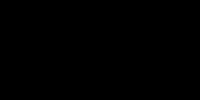
\includegraphics[width=0.3\textwidth]{../Images/gradient_x.png}
    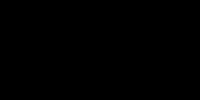
\includegraphics[width=0.3\textwidth]{../Images/gradient_y.png}
    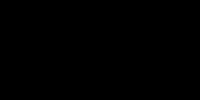
\includegraphics[width=0.3\textwidth]{../Images/gradient_magnitude.png}
    \caption{Computed gradients: (left) Gradient X, (middle) Gradient Y, (right) Gradient Magnitude}
    \label{fig:results}
\end{figure}

\section*{Conclusion}
This happens because when computing the gradient across channels, the strong increase in one channel can be canceled by a strong decrease in another. In this case, the red channel transitions from strong to zero, while the green channel transitions from zero to strong. When summed, these opposing gradients effectively nullify each other, resulting in a misleading overall gradient calculation.

This demonstrates the issue with summing individual color gradients. The results show that edges can be present in a color image while the summed gradient remains zero. Therefore we need an alternative gradient computation methods in color image processing.